% -----------------------------------------------------------------------------
%
% Copyright (c) 2017 Sam Cox, Roberto Sommariva
%
% This file is part of the AtChem2 software package.
%
% This file is covered by the MIT license which can be found in the file
% LICENSE.md at the top level of the AtChem2 distribution.
%
% -----------------------------------------------------------------------------

\chapter{Model Setup} \label{ch:setup}

% -------------------------------------------------------------------- %
\section{Chemical Mechanism} \label{sec:chemical-mechanism}

The chemical mechanism is the core of an atmospheric chemistry
model. In AtChem2, the chemical mechanism file is written in FACSIMILE
format and has the extension \texttt{.fac}. The FACSIMILE format is
used to describe chemical reactions in the commercial
\href{http://www.mcpa-software.com/}{FACSIMILE Kinetic Modelling Software};
for historical reasons, the software and the format have often
been used in conjunction with the MCM. The
\href{http://mcm.leeds.ac.uk/MCM/extract.htt}{extraction tool} on the
MCM website can generate \texttt{.fac} files in FACSIMILE format that
can be directly used in AtChem2 (Sect.~\ref{subsec:mcm-extraction}).

\subsection{FACSIMILE format} \label{subsec:facsimile-format}

Chemical reactions are described in FACSIMILE format using the
following notation:

\begin{verbatim}
% k : A + B = C + D ;
\end{verbatim}

where \texttt{k} is the rate coefficient, \texttt{A} and \texttt{B}
are the reactants, \texttt{C} and \texttt{D} are the products. A
reaction starts with the \texttt{\%} character and ends with the
\texttt{;} character. Comments can be inserted in the \texttt{.fac}
file to document and annotate the chemical mechanism: in FACSIMILE
format, comments are enclosed between the \texttt{*} and \texttt{;}
characters and are ignored by the compilation scripts.

The rate coefficient (\texttt{k}) is a constant number or, more
commonly, is calculated as a function of other variables, such as
temperature (\texttt{TEMP}), air density (\texttt{M}), water vapour
(\texttt{H2O}) and other environment variables
(Sect.~\ref{sec:environment-variables}). A basic chemical mechanism,
with comments and calculated rate coefficients, looks like this:

\begin{verbatim}
* Tropospheric O3-NOx cycle ;
* Kinetic data from Atkinson et al., ACP, 2004 ;
% J_NO2                      : NO2 = NO + O ;
% 5.6D-34*M*(TEMP/300)@-2.6  : O + O2 = O3 ;
% 1.4D-12*EXP(-1310/TEMP)    : NO + O3 = NO2 + O2 ;
\end{verbatim}

The photolysis rate of \cf{NO2} (\texttt{J\_NO2}) in the example above
is calculated by AtChem2 as function of latitude, longitude and solar
zenith angle (Sect.~\ref{subsec:calculated-photolysis-rates}).
Complex mathematical expressions can be used to calculate the rate
coefficients, in which case they have to be defined before the
chemical reactions that use them (typically, these are combination and
dissociation reactions). For example:

\begin{verbatim}
* Formation of nitric acid (HNO3) in the gas-phase ;
*;
* Rate coefficient (Atkinson et al., ACP, 2004) ;
K80 = 3.3D-30*M*(TEMP/300)@-3.0 ;
K8I = 4.1D-11 ;
KR8 = K80/K8I ;
FC8 = 0.4 ;
NC8 = 0.75-1.27*(LOG10(FC8)) ;
F8 = 10@(LOG10(FC8)/(1+(LOG10(KR8)/NC8)**2)) ;
KMT08 = (K80*K8I)*F8/(K80+K8I) ;
*;
* Chemical Reaction ;
% KMT08 : OH + NO2 = HNO3 ;
\end{verbatim}

Chemical reactions can be written in FACSIMILE format without
reactants or products. This feature can be used to implement simple
descriptions of non-chemical processes in a box-model. For example,
dilution (Sect.~\ref{subsec:dilute}), deposition to a surface, and
direct emission of a chemical species can be parametrized as:

\begin{verbatim}
* Deposition velocity of O3 = 1.4 cm s-1 ;
% 1.4/BLHEIGHT  :  O3 =  ;

* Emission rate of NO2 = 1e8 molecule cm-3 s-1 ;
% 1D+8  :  = NO2  ;
\end{verbatim}

More sophisticated approaches to describe non-chemical processes can
be implemented either by defining complex mathematical expressions to
calculate the corresponding ``rate coefficients'' (as explained above)
or by writing the appropriate Fortran function(s) into the source
code.

The \texttt{.fac} file is processed by a Python script
(\texttt{mech\_converter.py}, see Sect.~\ref{subsec:build-process}),
which expects the chemical mechanism to have four sections:

\begin{description}
\item[Generic rate coefficients] : contains the definitions of the
  generic rate coefficients used when experimental kinetic data are
  not available.
\item[Complex reactions] : contains the mathematical expressions used
  to calculate complex rate coefficients (e.g., for combination and
  dissociation reactions).
\item[Peroxy radicals] : contains the calculation of the \cf{RO2} sum
  -- go to Sect.~\ref{subsec:ro2-sum} for details.
\item[Reaction definitions] : contains the chemical reactions (and the
  parametrized non-chemical processes) in FACSIMILE format.
\end{description}

For \texttt{mech\_converter.py} to work, the beginning of each section
must be delimited by a header constituted by a single comment line.
The header must always be present, even though the corresponding
sections can be empty (e.g., if a mechanism other than the MCM is
used). A minimal \texttt{.fac} file (\texttt{mechanism\_skel.fac}) and
an example chemical mechanism downloaded from the MCM website
(\texttt{mechanism\_test.fac}) are included in the \texttt{mcm/}
directory for reference and testing.

\subsection{\cf{RO2} sum} \label{subsec:ro2-sum}

The sum of organic peroxy radicals (\cf{RO2}) is a key feature of the
Master Chemical Mechanism. Organic peroxy radicals react with
\cf{HO2}, with themselves and with other \cf{RO2}: given that there
are over 1000 peroxy radicals in the MCM, the number of possible self
and cross reactions of these species is of the order of $10^6$, which
presents a significant computational challenge. The \cf{RO2} sum is
used in the MCM to reduce the number of peroxy radicals permutation
reactions, as explained in the MCM protocol papers
\citep{jenkin_1997, saunders_2003}.

AtChem2 is designed primarily to run models based upon the MCM, and
therefore the \texttt{.fac} file must contain a section with the
calculation of the \cf{RO2} sum, as explained in
Sect.~\ref{subsec:facsimile-format}. This section must have a header
and has the following format:

\begin{verbatim}
* Peroxy radicals. ;
RO2 = RO2a + RO2b + RO2c + ... ;
\end{verbatim}

where \texttt{RO2a}, \texttt{RO2b}, \texttt{RO2c}, are the organic
peroxy radicals in the chemical mechanism. If there are no organic
peroxy radicals in the chemical mechanism (or if the mechanism is not
based upon the MCM), the \cf{RO2} sum section must still be present in
the \texttt{.fac} file, but it is left empty:

\begin{verbatim}
* Peroxy radicals. ;
RO2 = ;
\end{verbatim}

The \cf{RO2} sum is automatically generated from the chemical
mechanism during the build process using the list of \cf{RO2}
extracted from the MCM database (Sect.~\ref{subsec:build-process}).
AtChem2 includes the complete list of all organic peroxy radicals in
the MCM v3.3.1 (\texttt{mcm/peroxy-radicals\_v3.3.1}), which is the
version used by default. Complete lists of all organic peroxy radicals
in the other versions of the MCM are also included in the
\texttt{mcm/} directory. Instructions on how to set up AtChem2 to use
the previous versions of the MCM can be found in the file
\texttt{mcm/INFO.md}. The \cf{RO2} sum is output, by default, to the
file \texttt{environmentVariables.output} (Sect.~\ref{sec:output}).

It is important to ensure that the \cf{RO2} sum is accurate -- i.e.,
that it includes all the organic peroxy radicals in the chemical
mechanism -- because many reactions in the MCM depend on this
parameter. Note that the hydroperoxyl radical (\cf{HO2}) is a peroxy
radical but is not an organic molecule, and therefore it
\emph{should not be} included in the \cf{RO2} sum.

\subsection{MCM extraction} \label{subsec:mcm-extraction}

The MCM website provides a convenient tool that can be used to
download the whole Master Chemical Mechanism -- or subsets of it -- in
FACSIMILE format. Only a brief overview of the process is given here:
for more information go to the \href{http://mcm.leeds.ac.uk/}{MCM website}.

First, select the species of interest using the
\href{http://mcm.leeds.ac.uk/MCM/roots.htt}{MCM browser} and add the
selection to the ``Mark List''. Then proceed to the
\href{http://mcm.leeds.ac.uk/MCM/extract.htt}{MCM extraction tool} and
select the option ``FACSIMILE input format, suitable for inserting
into a FACSIMILE model''. Make sure that the following options are
selected, so that all the required headers
(Sect.~\ref{subsec:facsimile-format}) will be included in the
generated \texttt{.fac} file: :

\begin{verbatim}
[x] Include inorganic reactions?
[x] Include generic rate coefficients?
    FACSIMILE, FORTRAN and KPP formats only
\end{verbatim}

Click on the ``Extract'' button to download the \texttt{.fac} file
into a directory of choice -- such as the \texttt{model/} directory,
as discussed in Sect.~\ref{subsec:model-directory}. The downloaded
\texttt{.fac} file is a simple text file and is ready to be used in
AtChem2. If modifications are required (e.g., if some chemical
reactions have to be added, deleted or modified) open the
\texttt{.fac} file with a text editor and edit the chemical mechanism
as needed.

\subsection{The build process} \label{subsec:build-process}

AtChem2 is built using the scripts in the \texttt{build/}
directory. Here, we only outline the build process; detailed
instructions on how to build the model can be found in
Sect.~\ref{sec:build}.

The Python script \texttt{mech\_converter.py} -- automatically called
by the \texttt{build\_atchem2.sh} script -- converts the chemical
mechanism from the FACSIMILE format into a format that can be read by
the Fortran code. In doing so, the Python script generates a number of
files:

\begin{itemize}
\item \texttt{mechanism.f90} contains the equations, in Fortran code,
  to calculate the rate coefficients of each reaction of the chemical
  mechanism.
\item \texttt{mechanism.so} is the \textbf{shared library}, i.e. the
  pre-compiled version of the chemical mechanism.
\item \texttt{mechanism.species} contains the list of chemical species
  in the chemical mechanism. The file has no header. The first column
  is the \emph{ID number} of the species, the second column is the
  name of the species:
  \begin{verbatim}
  1 O
  2 O3
  3 NO
  4 NO2
  \end{verbatim}
\item \texttt{mechanism.reac} and \texttt{mechanism.prod} contain the
  reactants and the products (respectively) in each reaction of the
  chemical mechanism. The files have a one line header showing the
  number of species, the number of reactions and the number of
  equations in the \emph{Generic rate coefficients} and
  \emph{Complex reactions} sections (Sect.~\ref{subsec:facsimile-format}).
  The first column is the \emph{ID number} of the reaction, the second
  column is the \emph{ID number} of the chemical species (from
  \texttt{mechanism.species}) which are reactants/products in that
  reaction:
  \begin{verbatim}
  29 71 139 numberOfSpecies numberOfReactions numberOfGenericComplex
  1 1
  2 1
  3 1
  3 2
\end{verbatim}
\item \texttt{mechanism.ro2} contains the organic peroxy radicals
  (\cf{RO2}). The file has a one line header formatted as a Fortran
  comment. The first column is the \emph{ID number} of the peroxy
  radical (from \texttt{mechanism.species}), the second column is the
  name of the peroxy radical as a Fortran comment:
  \begin{verbatim}
  ! Note that this file is generated by build/mech_converter.py
  ! based upon the file mcm/mechanism_test.fac
  ! Any manual edits to this file will be overwritten when
  ! calling build/mech_converter.py
  23 !CH3O2
  26 !C2H5O2
  28 !IC3H7O2
  29 !NC3H7O2
  \end{verbatim}
\end{itemize}

In addition,                

The directory containing the files generated by the build script is
called \sharedir: by default, the \sharedir\ is in
\texttt{model/configuration/}, but its location can be changed using
the second argument of the build script, as explained in
Sect.~\ref{sec:build} (see also Sect.~\ref{subsec:model-directory}).

% -------------------------------------------------------------------- %
\section{Model Parameters} \label{sec:model-parameters}

The model parameters control the general setup of the model; they are
set in the \texttt{model.parameters} file which, by default, is
in the \texttt{model/configuration/} directory.

\begin{itemize}
\item \textbf{number of steps} and \textbf{step size}. The duration of
  the model run is determined by the number of steps and by the step
  size (in seconds). The step size controls the frequency of the model
  output for the chemical species listed in \texttt{outputSpecies.config}
  (Sect.~\ref{subsec:outputspecies}), as well as for the environment
  variables, the photolysis rates and the diagnostic variables. The
  step size is not related to the integration step which is controlled
  by CVODE.\\
  For example: a model runtime of 2 hours, with output every 5
  minutes, requires 24 steps with a step size of 300 seconds (24x300 =
  7200 sec = 2 hours).
\item \textbf{species interpolation method} and
  \textbf{conditions interpolation method}. Interpolation method used
  for the constrained chemical species, and for the constrained
  environment variables and the photolysis rates, respectively. Two
  interpolation methods are currently implemented in AtChem2:
  piecewise constant and piecewise linear
  (Sect.~\ref{subsec:interpolation}). The default option is \texttt{2}
  (piecewise linear interpolation).
\item \textbf{rates output step size}. Frequency (in seconds) of the
  model output for the production and loss rates of selected chemical
  species, i.e. those listed in \texttt{outputRates.config}
  (Sect.~\ref{sec:config-files}).
\item \textbf{model start time}. Start time of the model (in seconds)
  calculated from midnight of the \textbf{day}, \textbf{month},
  \textbf{year} parameters (see below). For example, a start time of
  3600 means the model run starts at 1:00 in the morning and a start
  time of 46800 means the model run starts at 1:00 in the afternoon
  (13:00). The \textbf{model stop time} is automatically calculated by
  the model as:
  \begin{verbatim}
  model start time + (number of steps * step size)
  \end{verbatim}
  \textit{N.B.}: when one or more variables are constrained, the time
  interval between the model start time and the model stop time
  \emph{must be} equal to or less than the time interval of the
  constrained data (Sect.~\ref{subsec:constraint-files} and
  Sect.~\ref{subsec:interpolation}).
\item \textbf{jacobian output step size}. Frequency (in seconds) of
  the model output for the Jacobian matrix. If this parameter is set
  to \texttt{0} (default option), the Jacobian matrix is not
  output.\\
  \textit{N.B.}: the \texttt{jacobian.output} file generated by the
  model can be very large, especially if the chemical mechanism has
  many reactions and/or the model runtime is long.
\item \textbf{latitude} and \textbf{longitude}. Geographical
  coordinates (in degrees). Latitude North is positive and latitude
  South is negative; longitude East is negative and longitude West is
  positive~\footnote{The standard geographical convention is that
    longitude East is positive and longitude West is negative. The
    current version of AtChem2 uses the opposite convention for
    backward compatibility reasons. This may change in future
    versions.}. Latitude and longitude are used to calculate the
  Earth-Sun angles, which are needed for the calculation of the
  photolysis rates (Sect.~\ref{subsec:calculated-photolysis-rates}).
\item \textbf{day} and \textbf{month} and \textbf{year}. Start date of
  the model simulation. The model time is in UTC (GMT timezone) and is
  calculated in seconds since midnight of the start date.
\item \textbf{reaction rates output step size}. Frequency (in seconds)
  of the model output for the reaction rates of every reaction in the
  chemical mechanism. By default, the reaction rates are saved in the
  directory \texttt{model/output/reactionRates/} as one file for each
  model step, with the name of the file corresponding to the time in
  seconds. In previous versions of AtChem, this output was called
  \textbf{instantaneous rates}. This parameter is different from
  \textbf{rates output step size} (see above), which sets the
  frequency of a formatted output of reaction rates for selected
  species of interest. For more information, go to
  Sect.~\ref{sec:config-files}.
\end{itemize}

% -------------------------------------------------------------------- %
\section{Solver Parameters} \label{sec:solver-parameters}

The solver parameters control the behaviour of the ordinary
differential equations (ODE) solver; they are set in the
\texttt{solver.parameters} file which, by default, is in the
\texttt{model/configuration/} directory. A complete explanation of
these parameters can be found in the documentation of the
\href{https://computation.llnl.gov/projects/sundials/sundials-software}{CVODE}
library.

\begin{itemize}
\item \textbf{atol} (positive real) and \textbf{rtol} (positive real):
  absolute and relative tolerance values for the solver.
\item \textbf{delta main} (positive real): linear convergence
  tolerance factor of the GMRES linear solver.
\item \textbf{lookback} (positive integer): maximum Krylov subspace
  dimension of the GMRES linear solver.
\item \textbf{maximum solver step size} (positive real): maximum size
  of the timesteps that the solver is allowed to use (in seconds).
\item \textbf{maximum number of steps in solver} (positive integer):
  maximum number of steps used by the solver before reaching
  \texttt{tout}, i.e. the next output time.
\item \textbf{solver type} (integer): selection of the linear solver
  to use: \texttt{1} for GMRES, \texttt{2} for GMRES preconditioned
  with a banded preconditioner (default option), \texttt{3} for a
  dense solver.
\item \textbf{banded preconditioner upper bandwidth} (integer): only
  used in the case that \texttt{solver\ type\ =\ 2}.
\item \textbf{banded preconditioner lower bandwidth} (integer): only
  used in the case that \texttt{solver\ type\ =\ 2}.
\end{itemize}

% -------------------------------------------------------------------- %
\section{Environment Variables} \label{sec:environment-variables}

The environment variables define the physical parameters of the model,
such as temperature, pressure, humidity, latitude, longitude, position
of the sun, etc\ldots. These variables are set in the
\texttt{environmentVariables.config} file which, by default, is in the
\texttt{model/configuration/} directory.

The environment variables can have a fixed (constant) value or can be
constrained to measured values (\texttt{CONSTRAINED}), in which case
the corresponding data file must be present in the
\texttt{model/constraints/environment/} directory
(Sect.~\ref{subsec:constraint-files}). Some environment variables can
be calculated by the model (\texttt{CALC}) and some can be deactivated
if they are not needed (\texttt{NOTUSED}).

By default, the environment variables are set either to \texttt{NOTUSED} or
to a fixed value. The AtChem2 environment variables are described
below, together with their possible settings, units, and their default
values.

\subsection{TEMP} \label{subsec:temp}

Ambient Temperature (K).

\begin{itemize}
\item fixed value
\item constrained
\end{itemize}

Default fixed value = 298.15

\subsection{PRESS} \label{subsec:press}

Ambient Pressure (mbar).

\begin{itemize}
\item fixed value
\item constrained
\end{itemize}

Default fixed value = 1013.25

\subsection{RH} \label{subsec:rh}

Relative Humidity (\%). It is required only if
\hyperref[subsec:h2o]{\texttt{H2O}} is set to \texttt{CALC}, otherwise
it must be set to \texttt{NOTUSED}.

\begin{itemize}
\item fixed value
\item constrained
\item not used
\end{itemize}

Default = NOTUSED (-1)

\subsection{H2O} \label{subsec:h2o}

Water Concentration (molecule cm$^{-3}$). If \texttt{H2O} is set to
\texttt{CALC}, then \hyperref[subsec:rh]{\texttt{RH}} must be set to a
fixed value or to \texttt{CONSTRAINED}.

\begin{itemize}
\item fixed value
\item constrained
\item calculated
\end{itemize}

Default fixed value = 3.91e+17

\subsection{DEC} \label{subsec:dec}

Sun Declination (radians) is the angle between the center of the Sun
and Earth's equatorial plane.

\begin{itemize}
\item fixed value
\item constrained
\item calculated
\end{itemize}

Default fixed value = 0.41

\subsection{BLHEIGHT} \label{subsec:blheight}

Boundary Layer Height. It is required only if the model includes
non-chemical processes, such as emission or deposition of chemical
species. The unit is usually centimetre or metre, depending on how
these processes are parametrized in the chemical mechanism -- go to
Sect.~\ref{subsec:facsimile-format} for details.

\begin{itemize}
\item fixed value
\item constrained
\item not used
\end{itemize}

Default = NOTUSED (-1)

\subsection{DILUTE} \label{subsec:dilute}

Dilution rate (s$^{-1}$). It is required only if the model includes
dilution of the chemical species. If \texttt{DILUTE} is set to a fixed
value, the chemical mechanism is automatically modified during the
\hyperref[subsec:build-process]{build process}: for each species in
the chemical mechanism, a loss ``reaction'' is added to the mechanism
with a ``rate coefficient'' equal to the dilution rate. For example,
the following is added to the \emph{Tropospheric O3-NOx cycle}
chemical mechanism shown in Sect.~\ref{subsec:facsimile-format}:

\begin{verbatim}
% DILUTE : NO2 = ;                  
% DILUTE : NO = ;
% DILUTE : O = ;
% DILUTE : O3 = ;
\end{verbatim}

The new set of reactions~\footnote{Molecular oxygen (\cf{O2}) and
  nitrogen (\cf{N2}) are treated in AtChem2 as model parameters, not
  as chemical species, and their concentrations are calculated as a
  function of temperature and pressure. Therefore, \texttt{DILUTE} is
  not applied to \cf{O2} and \cf{N2}} effectively emulates the
dilution of the chemical system. \texttt{DILUTE} cannot be
constrained.

\begin{itemize}
\item fixed value
\item not used
\end{itemize}

Default value = NOTUSED (-1)

\subsection{JFAC} \label{subsec:jfac}

Correction factor used to adjust the photolysis rates -- e.g., to
account for the presence of clouds. \texttt{JFAC} can have a value
between \texttt{0} (photolysis rates are set to zero) and \texttt{1}
(photolysis rates are not corrected). JFAC is \emph{not applied} to
constant or constrained photolysis rates (Fig.~\ref{fig:photol}). For
more information go to Sect.~\ref{subsec:jfac-calculation}.

\begin{itemize}
\item fixed value
\item constrained
\item calculated
\end{itemize}

Default fixed value = 1

\subsection{ROOF} \label{subsec:roof}

Flag to switch the photolysis rates on/off. It is needed mostly for
simulations of some environmental chamber experiments, where the roof
of the chamber can be opened/closed or the lamps can be turned on/off.

When \texttt{ROOF} is set to \texttt{CLOSED} all the photolysis rates
are set to zero, including those that are constant or constrained:
this is different than setting \texttt{JFAC} to \texttt{0}, which only
applies to the calculated photolysis rates (Fig.~\ref{fig:photol}).

\texttt{ROOF} is can be set only to \texttt{OPEN} (default) or
\texttt{CLOSED} and cannot be constrained.

% -------------------------------------------------------------------- %
\section{Photolysis Rates} \label{sec:photolysis-rates}

The photolysis rates are identified in
\hyperref[subsec:facsimile-format]{FACSIMILE format} with the notation
\verb|J<n>|, where \texttt{n} is an integer assigned by the MCM to
each photolysis reaction (or to a group of photolysis reactions). By
default, AtChem2 calculates the photolysis rates using the MCM
\href{http://mcm.leeds.ac.uk/MCM/parameters/photolysis_param.htt}{parametrization},
which is described in Sect.~\ref{subsec:calculated-photolysis-rates}.
Each photolysis rate can also be set to a constant value or
constrained to measured data. The following rules apply:

\begin{enumerate}
\item If a photolysis rate is set as constant, it assumes the given
  value; the other photolysis rates are set to zero.
\item If a photolysis rate is constrained, it assumes the values in
  the corresponding constraint file; the other photolysis rates are
  calculated.
\item If no photolysis rate is set to constant or constrained, the
  model calculates all photolysis rates.
\end{enumerate}

Fig.~\ref{fig:photol} shows in detail how AtChem2 combines constant,
constrained and calculated photolysis rates, as well as the usage of
the correction factor JFAC (Sect.~\ref{subsec:jfac-calculation}).
Additionally, the environment variable \texttt{ROOF} can be used to
turn the photolysis rates ON or OFF, as explained in
Sect.~\ref{subsec:roof}.

\begin{figure}[htb]
  \centering
  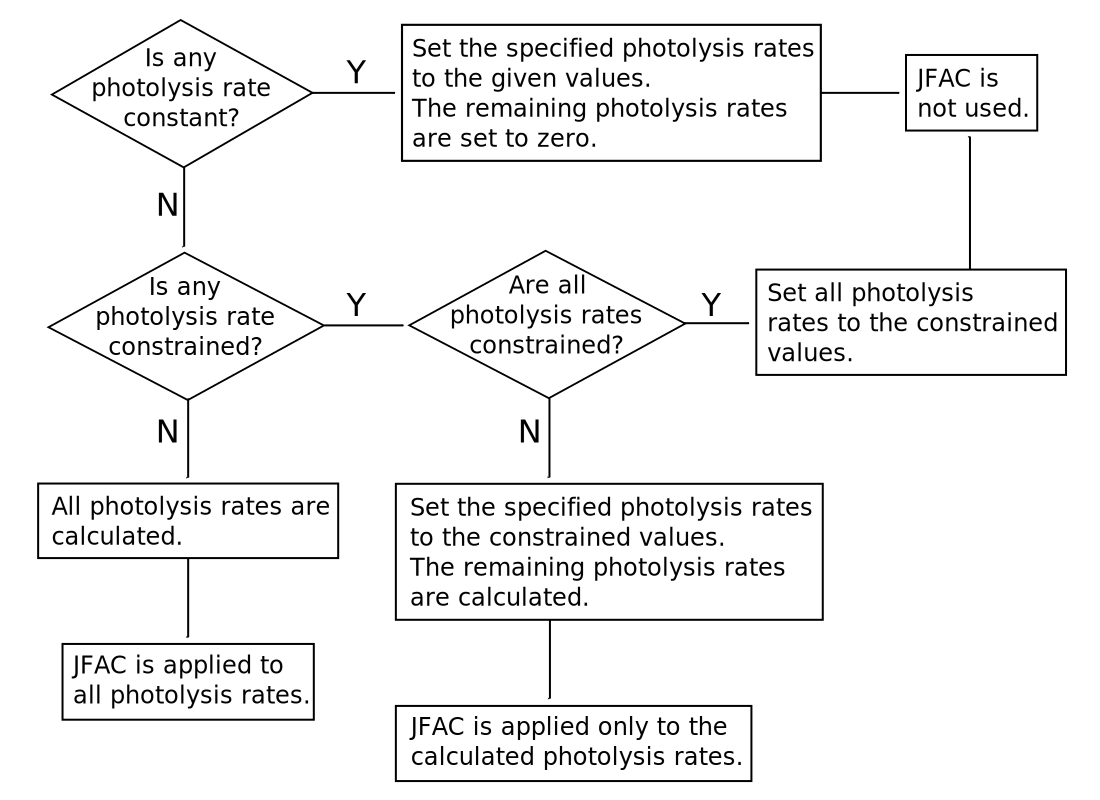
\includegraphics[width=0.8\textwidth]{photolysis-rates.png}
  \caption{Treatment of photolysis rates in AtChem2.} \label{fig:photol}
\end{figure}

\subsection{Constant photolysis rates} \label{subsec:constant-photolysis-rates}

The typical scenario for constant photolysis rates is a lamp or solar
simulator in an environmental chamber. All the photolysis rates in the
chemical mechanism must be given a value in the
\texttt{photolysisConstant.config} file, otherwise they are
automatically set to zero (Fig.~\ref{fig:photol}). If the file is
empty, the photolysis rates are calculated (or constrained, see
below). This allows the user to model individual photolysis processes
and/or to account for lamps that emit only in certain spectral
windows. The format of the \texttt{photolysisConstant.config} file is
described in Sect.~\ref{subsec:photolysisconstant}.

\subsection{Constrained photolysis rates} \label{subsec:constrained-photolysis-rates}

All photolysis rates can be constrained to measured values. In this
case, the name of the constrained photolysis rate (e.g., \texttt{J2})
must be listed in \texttt{photolysisConstrained.config}
(Sect.~\ref{subsec:photolysisconstrained}) and a corresponding file
with the constraint data must be present in the
\texttt{model/constraints/photolysis/} directory
(Sect.~\ref{subsec:constraint-files}).                            

It is not always possible to measure -- and therefore constrain -- all
the required photolysis rates. The photolysis rates that are not
constrained (i.e., not listed in \texttt{photolysisConstrained.config})
are calculated using the MCM parametrization, described in the next
section.

\subsection{Calculated photolysis rates} \label{subsec:calculated-photolysis-rates}

AtChem2 implements the parametrization of photolysis rates used by the
Master Chemical Mechanism, which is described in the MCM protocol
papers \citep{jenkin_1997, saunders_2003}. Briefly, the photolysis
rate (\texttt{J}) of a reaction is calculated as a function of the
solar zenith angle with the equation:

\begin{verbatim}
J = l * (cosX)^m * exp(-n * secX) * tau
\end{verbatim}

where \texttt{l}, \texttt{m}, \texttt{n} are empirical parameters,
\texttt{cosX} is the cosine of the solar zenith angle, \texttt{secX}
is the inverse of \texttt{cosX} (i.e., \texttt{secX\ =\ 1/cosX}) and
\texttt{tau} is the transmission factor. The empirical parameters are
different for each version of the MCM \citep{sommariva_2019}. AtChem2
includes the empirical parameters for the MCM v3.3.1
(\texttt{mcm/photolysis-rates\_v3.3.1}). It is possible to use
previous versions of the MCM parametrization and to change the value
of \texttt{tau}: see the file \texttt{mcm/INFO.md} for
instructions. The transmission factor \texttt{tau} can be used to
account for the loss of natural or artificial light in some
environmental chambers and is by default set to 1 (i.e., perfect
trasmittance of the chamber walls).

The solar zenith angle (SZA) is the angle between the local vertical
and the center of the Sun, in radians. The SZA is calculated by
AtChem2 using the environment variables latitude, longitude, sun
declination (Sect.~\ref{sec:environment-variables}), and the time of
the day. The calculation of the sun declination -- if not constrained
or set to a constant values -- and of the solar zenith angle is
described in \citet{madronich_1993}.

\subsection{JFAC calculation} \label{subsec:jfac-calculation}

Measurements of ambient photolysis rates typically show short-term
variability due to the changing meteorological conditions, such as
clouds, rain, aerosol, etc\ldots. This information is retained in the
constrained photolysis rates, but it is lost in the calculated
ones. To account for ambient variability, the calculated photolysis
rates can be scaled by a constant or time-dependent correction factor,
the environment variable \texttt{JFAC} (Sect.~\ref{subsec:jfac}).

\texttt{JFAC} is defined as the ratio between a measured and a
calculated photolysis rate. Typically, \texttt{J4} -- the photolysis
rate of \cf{NO2} -- is used for this purpose, because it is one of the
most frequently measured photolysis rates:

\begin{verbatim}
JFAC = j(NO2)/J4
\end{verbatim}

where \texttt{j(NO2)} is measured and \texttt{J4} is calculated with
the MCM parametrization (Sect.~\ref{subsec:calculated-photolysis-rates}).

\texttt{JFAC} is by default set to 1, meaning that the calculated
photolysis rates are not scaled; it can be set to any value between 0
and 1 (Sect.~\ref{subsec:jfac}) or it can be constrained
(Sect.~\ref{subsec:constrained-variables}). Note that only the
photolysis rates calculated with the MCM parametrization are scaled by
\texttt{JFAC}, while the constrained and the constant photolysis rates
are never scaled (Fig.~\ref{fig:photol}).

\texttt{JFAC} can also be calculated by AtChem2 at runtime. To use
this option, edit \texttt{environmentVariables.config} and set
\texttt{JFAC} to the name of the photolysis rate used as reference
(e.g., \texttt{J4}). The reference photolysis rate should be
constrained -- i.e., listed in \texttt{photolysisConstrained.config}
(Sect.~\ref{subsec:photolysisconstrained}) -- and the corresponding
constraint file present in the \texttt{model/constraints/environment/}
directory~\footnote{\textit{N.B.}: the calculation of \texttt{JFAC} at
  runtime does not work well in the current version of AtChem2,
  especially when the reference photolysis rate is very
  variable. Therefore, it is recommended to calculate \texttt{JFAC}
  offline and then to constrain it (see issue
  \href{https://github.com/AtChem/AtChem2/issues/16}{\#16})}.

% -------------------------------------------------------------------- %
\section{Config Files} \label{sec:config-files}

The configuration files contain the settings of the environment
variables, the chemical species, and the photolysis rates, as well as
the model constraints and the model output. All the configuration
files have the extension \texttt{.config} and, by default, are located
in the \texttt{model/configuration/} directory. This directory also
contains the files with the settings of the model (in
\texttt{model.parameters}) and of the solver (in
\texttt{solver.parameters}), which are described in
Sect.~\ref{sec:model-parameters} and Sect.~\ref{sec:solver-parameters}.
Usually, the \texttt{model/configuration/} directory is also the
\sharedir, which contains the chemical mechanism files generated
during the \hyperref[subsec:build-process]{build process}.

The location of these directories can be modified by the user, as
explained in Sect.~\ref{subsec:model-directory}). The content and the
format of each \texttt{.config} file are described below. Note that
the names of some files have changed with the release of AtChem2
version 1.1 (November 2018).

\subsection{environmentVariables.config} \label{subsec:environmentvariables}

This file contains the settings of the environment variables
(Sect.~\ref{sec:environment-variables}. The file has three columns:
the first two are the \emph{ID number} and the name of each
environment variable. The third column, which is the only one that
should be modified by the user, contains the settings of the
environment variables. For example:

\begin{verbatim}
1 TEMP            293
2 PRESS           1013
3 RH              CONSTRAINED
4 H2O             CALC
5 DEC             CALC
6 BLHEIGHT        8e+4
7 DILUTE          NOTUSED
8 JFAC            CONSTRAINED
9 ROOF            OPEN
\end{verbatim}

If an environment variable is constrained, there must be a
corresponding data file in the \texttt{model/constraints/environment/}
directory (Sect.~\ref{sec:constraints}).

\subsection{initialConcentrations.config} \label{subsec:initialconcentrations}

This file contains the initial concentrations of the chemical species
-- in molecule cm$^{-3}$. The file has two columns: the first column
is the list of initialized species, the second column is the
corresponding concentration at \texttt{t\ =\ 0}. For example:

\begin{verbatim}
NO      378473308.14
NO2     86893908168.9
O3      1.213e+12
CH4     4.938e+13
\end{verbatim}

Not all chemical species need to be initialized: those that are not
listed in \texttt{initialConcentrations.config} are automatically set
to an initial concentration of \texttt{0.0e+00} molecule cm$^{-3}$. It
is not necessary to initialize the chemical species that are set to
constant or constrained -- i.e., those listed in
\texttt{speciesConstant.config} or in \texttt{speciesConstrained.config}
(see below).

\subsection{outputRates.config} \label{subsec:outputrates}

This file lists the chemical species for which detailed production and
loss rates are required. In version 1.0 and earlier, these species
were listed in two files called \texttt{productionRatesOutput.config}
and \texttt{lossRatesOutput.config}. The file has one column, with one
species per line.

The frequency of this output is controlled by the
\textbf{rates output step size} parameter in \texttt{model.parameters}
(Sect.~\ref{sec:model-parameters}). The corresponding output files --
called \texttt{productionRates.output} and \texttt{lossRates.output}
-- are designed to facilitate the analysis of the production and
destruction rates of selected species of interests, rather than
processing all the files saved in the
\texttt{model/output/reactionRates/} directory. For more information
go to Sect.~\ref{sec:output}.

\subsection{outputSpecies.config} \label{subsec:outputspecies}

This file (called \texttt{concentrationOutput.config} in version 1.0
and earlier) lists the chemical species for which the calculated
concentration -- molecule cm$^{-3}$ -- is required. The current
version of AtChem2 limits the number of species that can be output to
100, although the user can modify the Fortran
code~\footnote{Subroutine \texttt{outputSpeciesOfInterest()} in
  \texttt{src/outputFunctions.f90} controls the output of the chemical
  species.} to increase this number. The file has one column, with one
species per line.

The frequency of this output is controlled by the \textbf{step size}
parameter in \texttt{model.parameters} (Sect.~\ref{sec:model-parameters}).
The constrained chemical species can be listed in
\texttt{outputSpecies.config}, which is sometimes useful for
diagnostic and debugging. Note that the photolysis rates, the
environment variables and the \cf{RO2} sum are always output by the
model (Sect.~\ref{sec:output}) and therefore there is not an
equivalent config file for the output of these variables.

\subsection{photolysisConstant.config} \label{subsec:photolysisconstant}

This file lists the photolysis rates that are set to constant
(Sect.~\ref{subsec:constant-photolysis-rates}). The file has three
columns: the first column is the number that identifies the photolysis
rate (e.g., \texttt{1}), the second column is the value of the
photolysis rate in s$^{-1}$ (e.g., \texttt{1e-5}), the third column is
the name of the photolysis rate (e.g., \texttt{J1}). The photolysis
rates are named according to the MCM
\href{http://mcm.leeds.ac.uk/MCM/parameters/photolysis.htt}{naming convention}
(Sect.~\ref{sec:photolysis-rates}).

If no photolysis rate is set to constant, the file should be empty.
The photolysis rates that are not listed in \texttt{photolysisConstants.config}
are automatically set to zero (Fig.~\ref{fig:photol}).

\subsection{photolysisConstrained.config} \label{subsec:photolysisconstrained}

This file (called \texttt{constrainedPhotoRates.config} in version 1.0
and earlier) lists the photolysis rates that are constrained
(Sect.~\ref{subsec:constrained-photolysis-rates}). The file has one
column, with one photolysis rate per line (e.g., \texttt{J1}). The
photolysis rates are named according to the MCM
\href{http://mcm.leeds.ac.uk/MCM/parameters/photolysis.htt}{naming convention}
(Sect.~\ref{sec:photolysis-rates}). If a photolysis rate is
constrained, there must be a corresponding data file in the
\texttt{model/constraints/photolysis/} directory
(Sect.~\ref{subsec:constrained-variables}).

If no photolysis rate is constrained, the file should be empty. The
photolysis rates that are not listed in \texttt{photolysisConstrained.config}
are calculated using the MCM parametrization (Fig.~\ref{fig:photol}).

\subsection{speciesConstant.config} \label{subsec:speciesconstant}

This file (called \texttt{constrainedFixedSpecies.config} in version
1.0 and earlier) lists the chemical species that are set to
constant. The file has two columns: the first column is the list of
constant species, the second column is the corresponding concentration
-- in molecule cm$^{-3}$.

If no chemical species is set to constant, the file should be empty.
The chemical species that are set to a constant value do not need to
be initialized: the values set in \texttt{speciesConstant.config}
override those set in \texttt{initialConcentrations.config}.

\subsection{speciesConstrained.config} \label{subsec:speciesconstrained}

This file (called \texttt{constrainedSpecies.config} in version 1.0
and earlier) lists the chemical species that are constrained. The file
has one column, with one species per line. If a chemical species is
constrained, there must be a corresponding data file in the
\texttt{model/constraints/species/} directory
(Sect.~\ref{subsec:constrained-variables}).

If no chemical species is constrained, the file should be empty. The
chemical species that are constrained do not need to be initialized:
the values set in \texttt{speciesConstrained.config} override those
set in \texttt{initialConcentrations.config}.
